
\subsubsection{ee}

\begin{figure}[htb!]
    \centering
    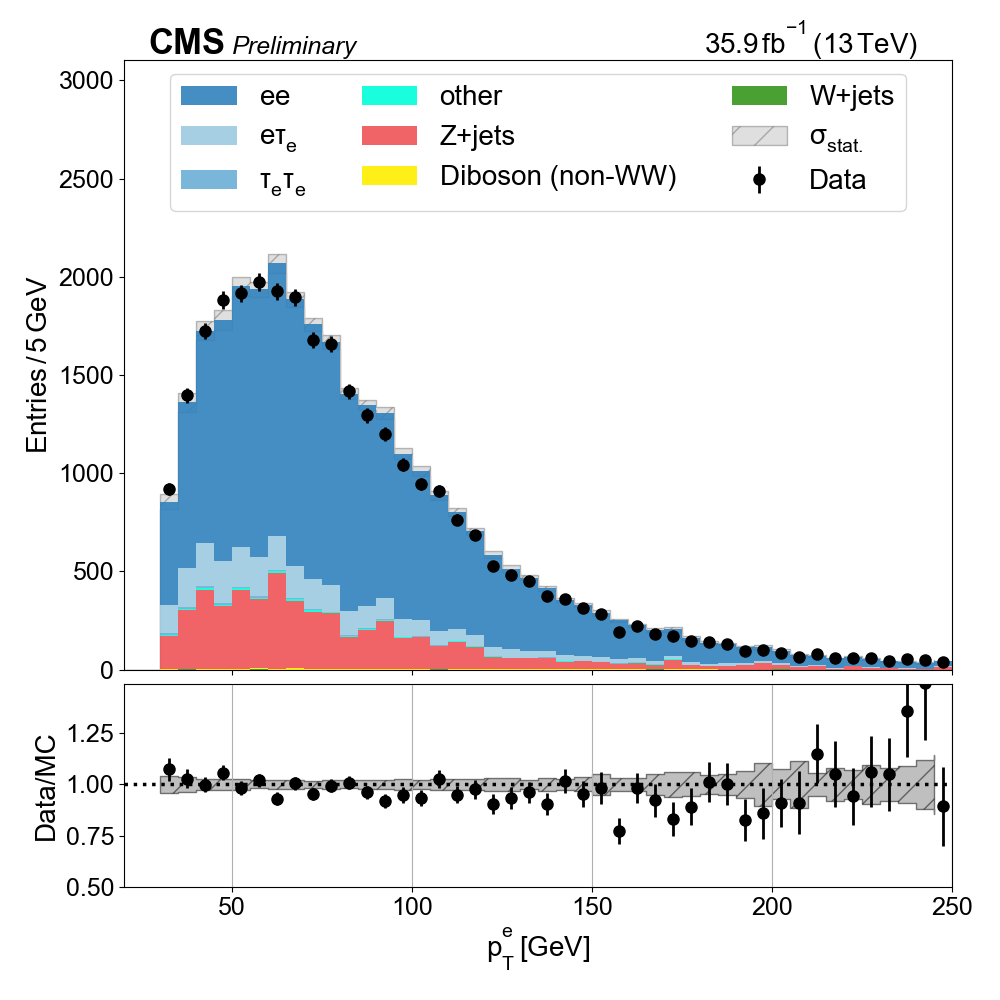
\includegraphics[width=0.4\textwidth]{chapters/Analysis/sectionPlots/figures/data_mc_overlays/ee_2016_cat_gt2_eq1_b_signal_linear_lepton_lepton1_pt}
    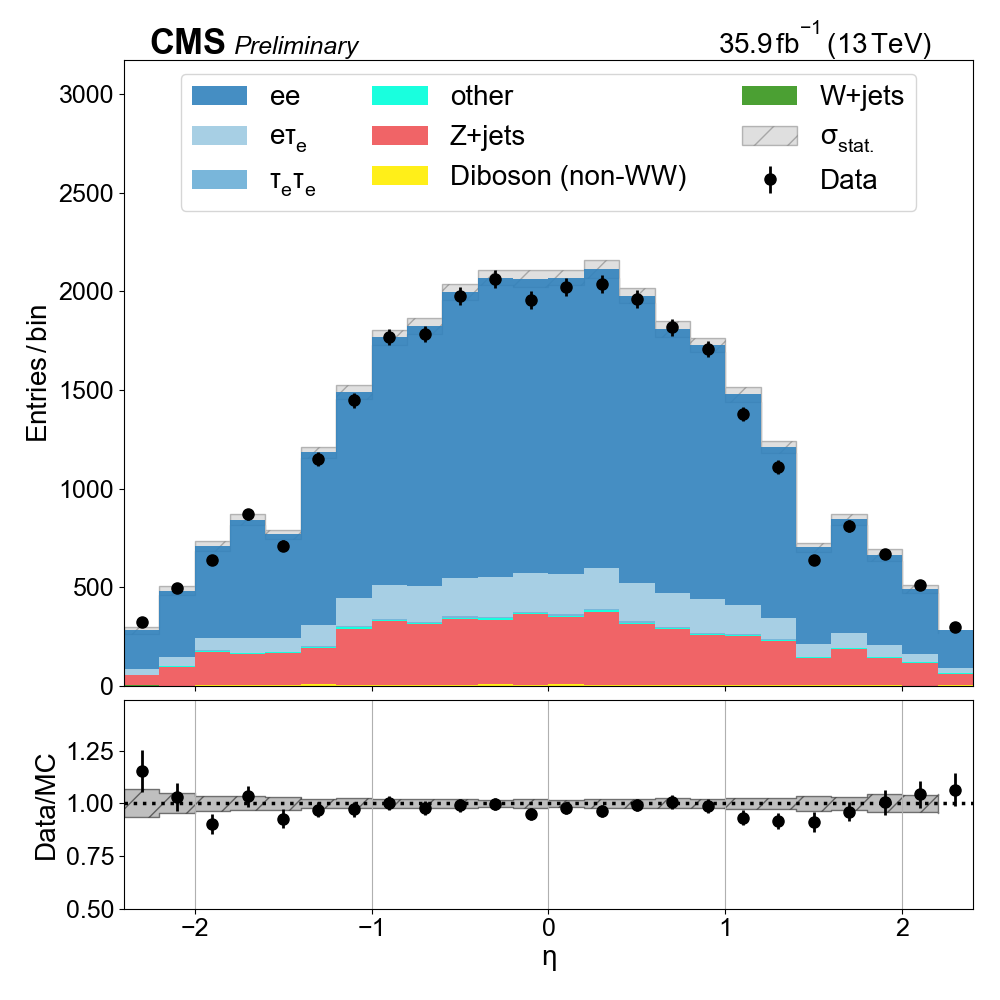
\includegraphics[width=0.4\textwidth]{chapters/Analysis/sectionPlots/figures/data_mc_overlays/ee_2016_cat_gt2_eq1_b_signal_linear_lepton_lepton1_eta}

    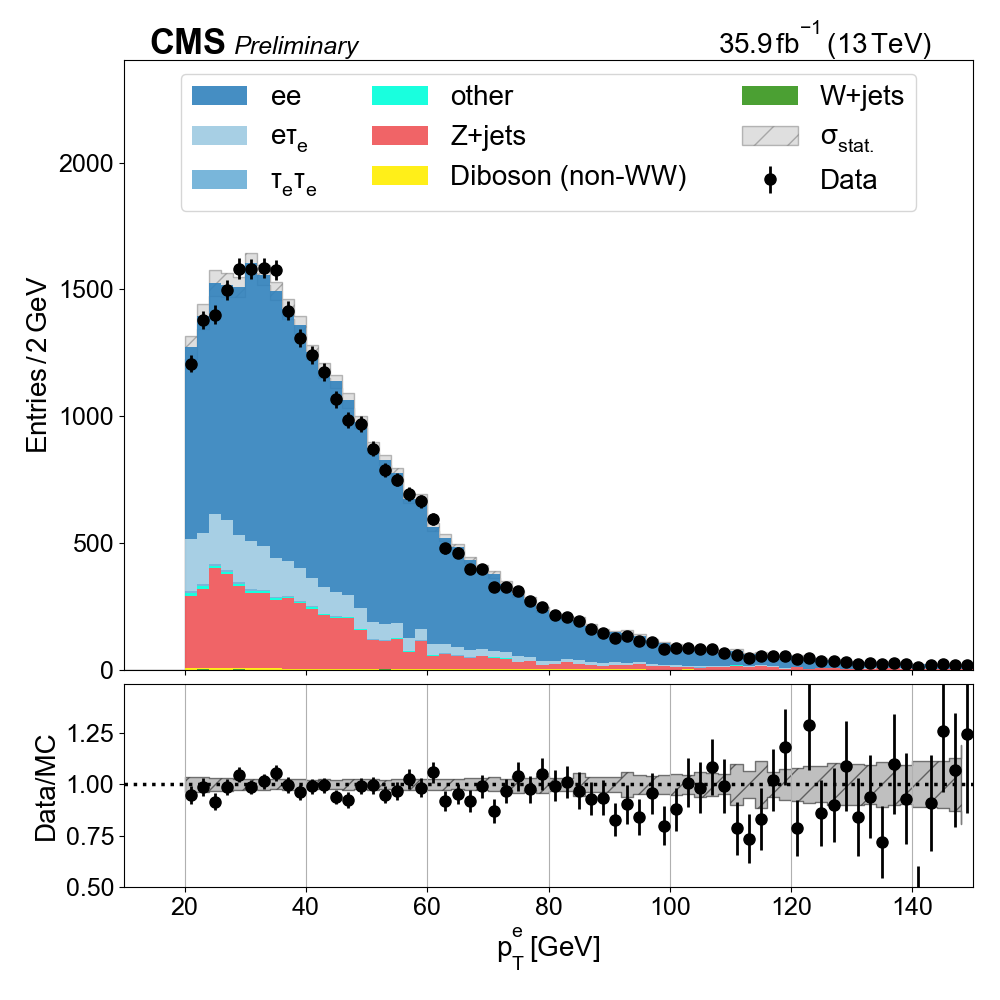
\includegraphics[width=0.4\textwidth]{chapters/Analysis/sectionPlots/figures/data_mc_overlays/ee_2016_cat_gt2_eq1_b_signal_linear_lepton_lepton2_pt}
    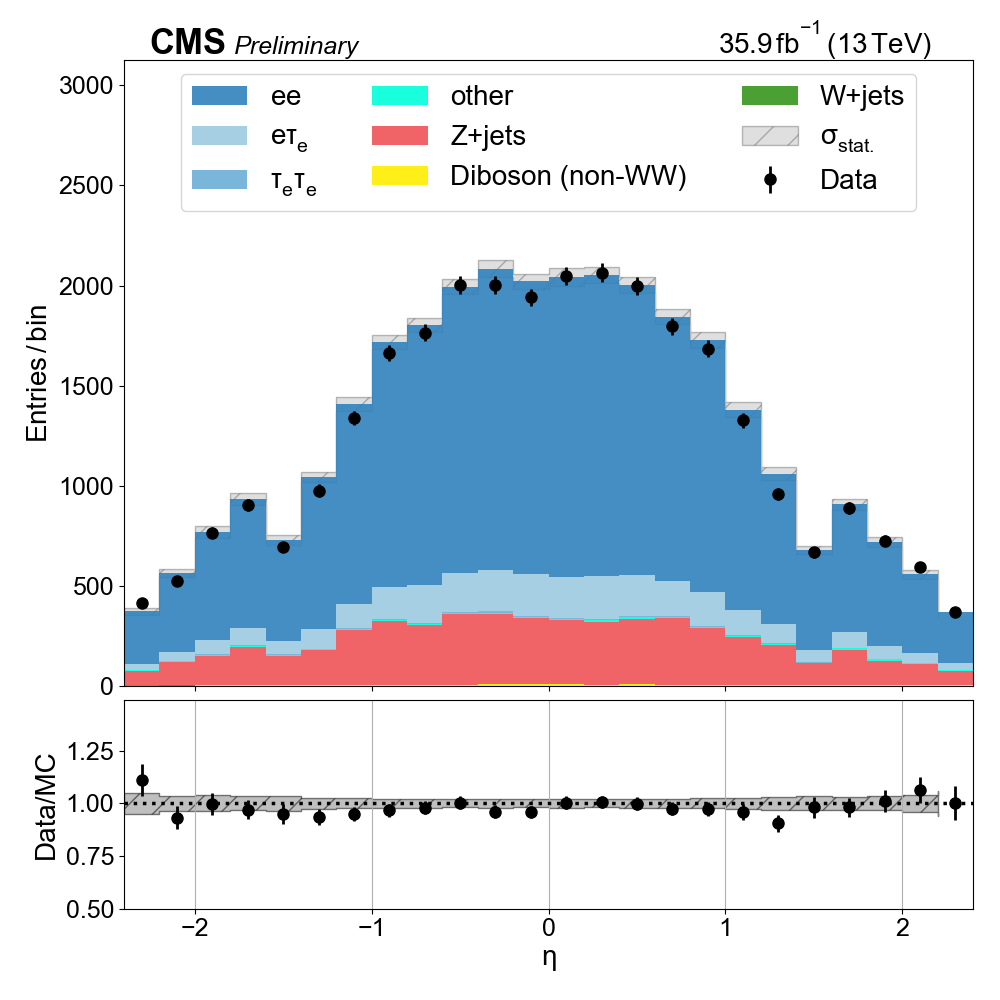
\includegraphics[width=0.4\textwidth]{chapters/Analysis/sectionPlots/figures/data_mc_overlays/ee_2016_cat_gt2_eq1_b_signal_linear_lepton_lepton2_eta}
    \caption{\pt and $\eta$ distributions for leading (top) and trailing
    (bottom) electrons in the $ee$ channel with $N_{j} \geq 2$, $N_{b}
    = 1$, and Z boson veto.}
    \label{fig:analysis:plots:ee_1_kinematic}
\end{figure}

\begin{figure}[htb!]
    \centering
    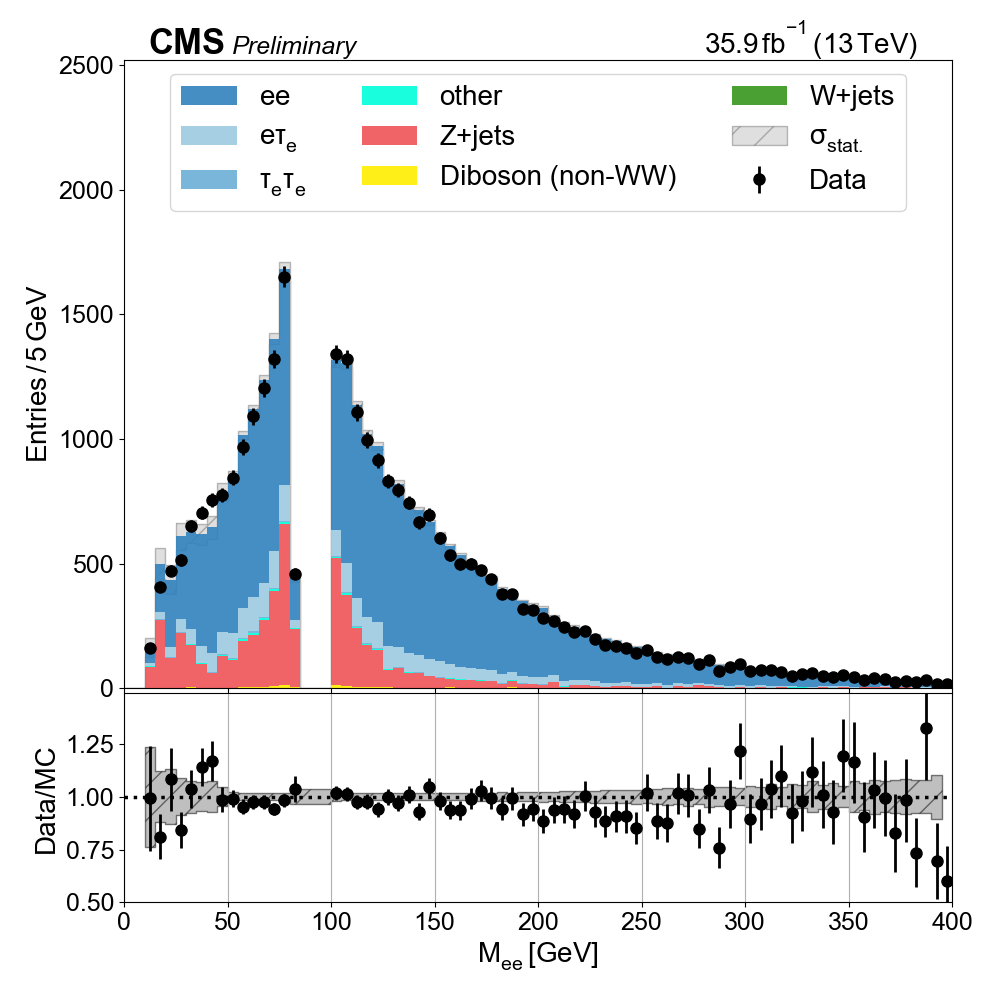
\includegraphics[width=0.3\textwidth]{chapters/Analysis/sectionPlots/figures/data_mc_overlays/ee_2016_cat_gt2_eq1_b_signal_linear_lepton_dilepton1_mass}
    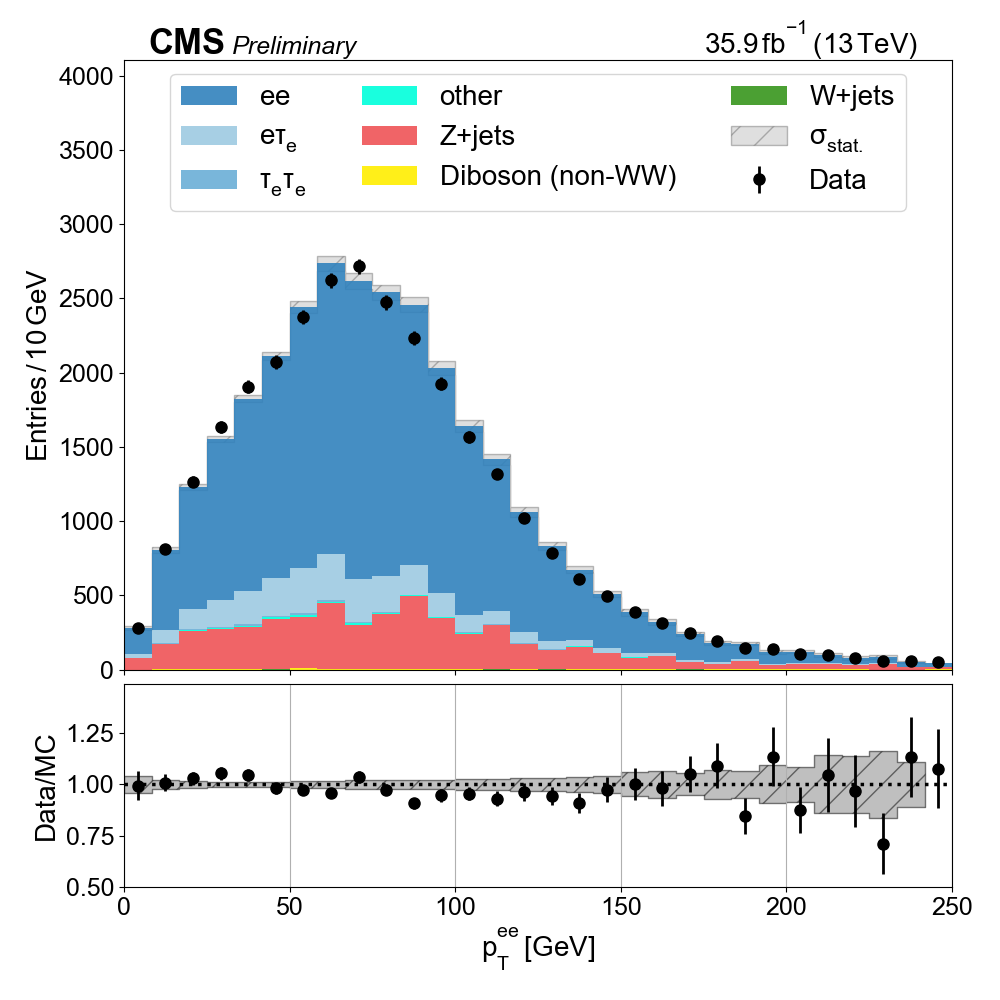
\includegraphics[width=0.3\textwidth]{chapters/Analysis/sectionPlots/figures/data_mc_overlays/ee_2016_cat_gt2_eq1_b_signal_linear_lepton_dilepton1_pt}
    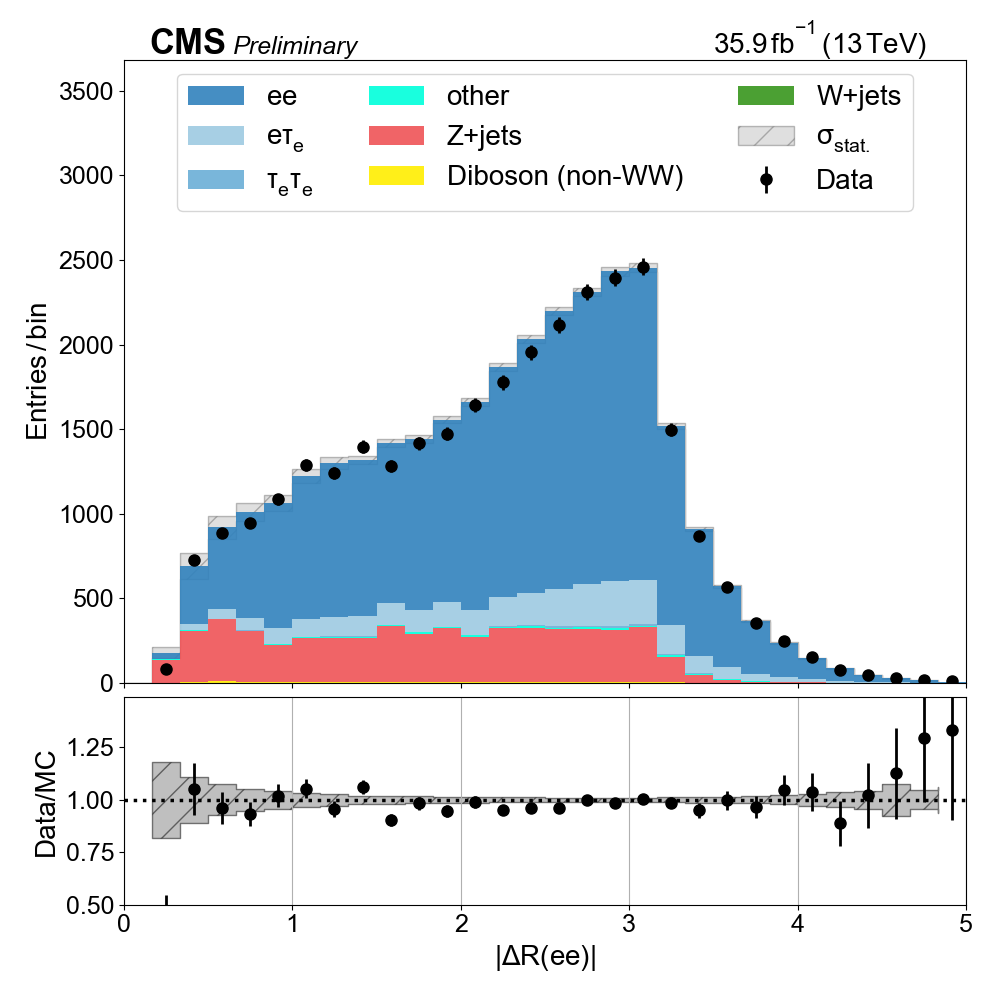
\includegraphics[width=0.3\textwidth]{chapters/Analysis/sectionPlots/figures/data_mc_overlays/ee_2016_cat_gt2_eq1_b_signal_linear_lepton_dilepton1_delta_r}
    \caption{Dielectron mass, \pt, and $\Delta R$ in the $ee$ channel
    with $N_{j} \geq 2$, $N_{b} = 1$, and Z boson veto.}
    \label{fig:analysis:plots:ee_1_dilepton}
\end{figure}

\begin{figure}[htb!]
    \centering
    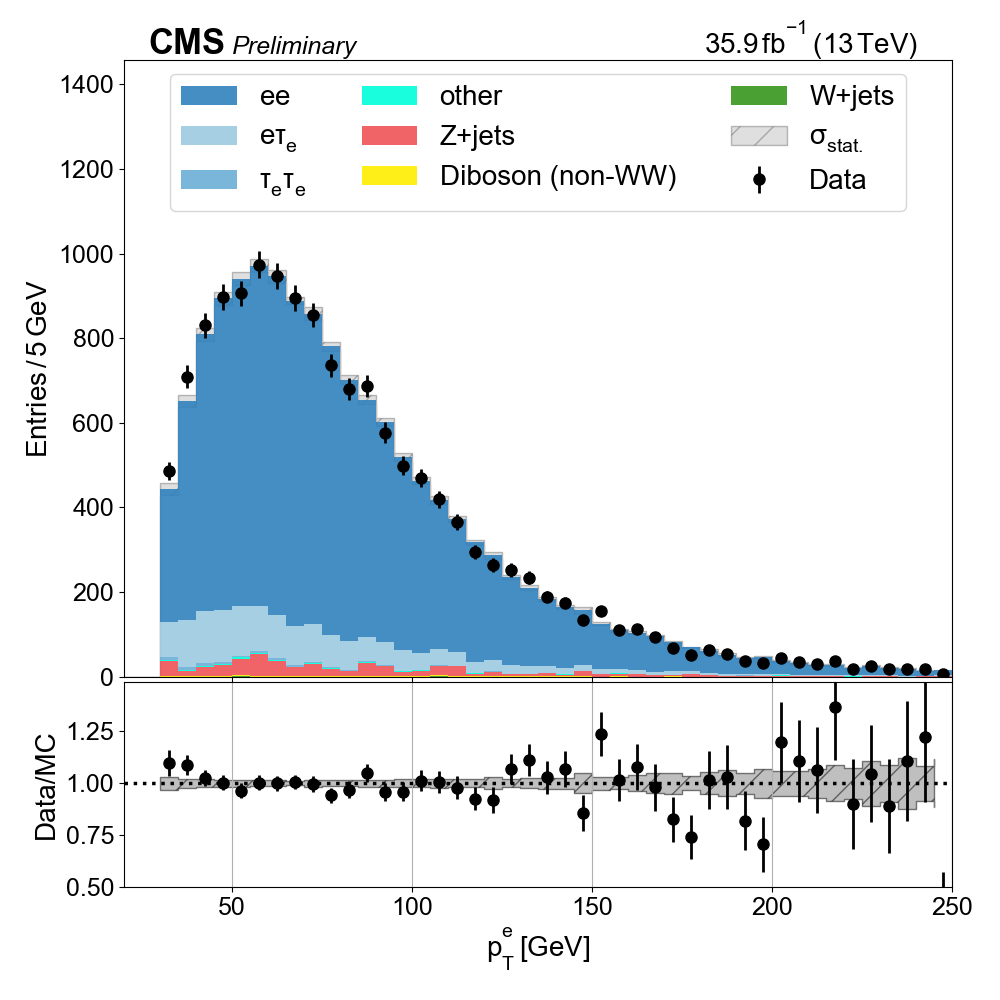
\includegraphics[width=0.4\textwidth]{chapters/Analysis/sectionPlots/figures/data_mc_overlays/ee_2016_cat_gt2_gt2_b_signal_linear_lepton_lepton1_pt}
    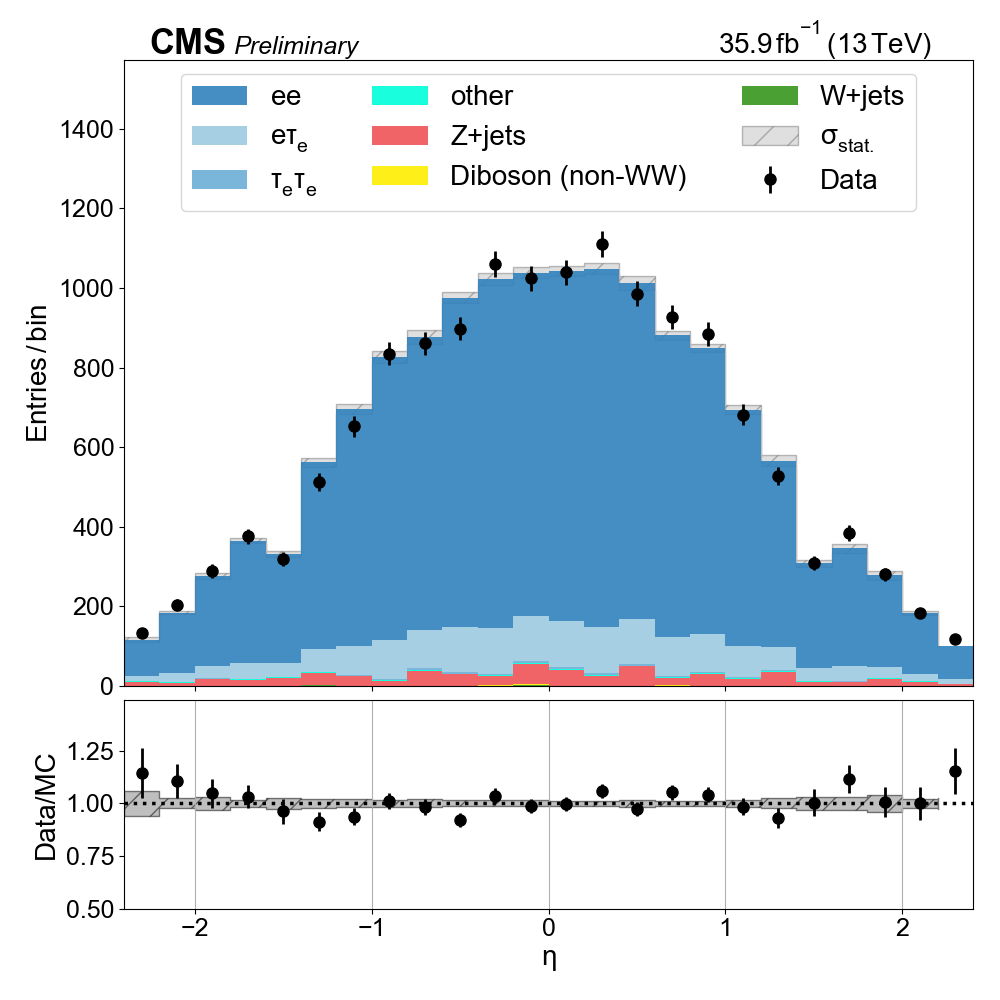
\includegraphics[width=0.4\textwidth]{chapters/Analysis/sectionPlots/figures/data_mc_overlays/ee_2016_cat_gt2_gt2_b_signal_linear_lepton_lepton1_eta}

    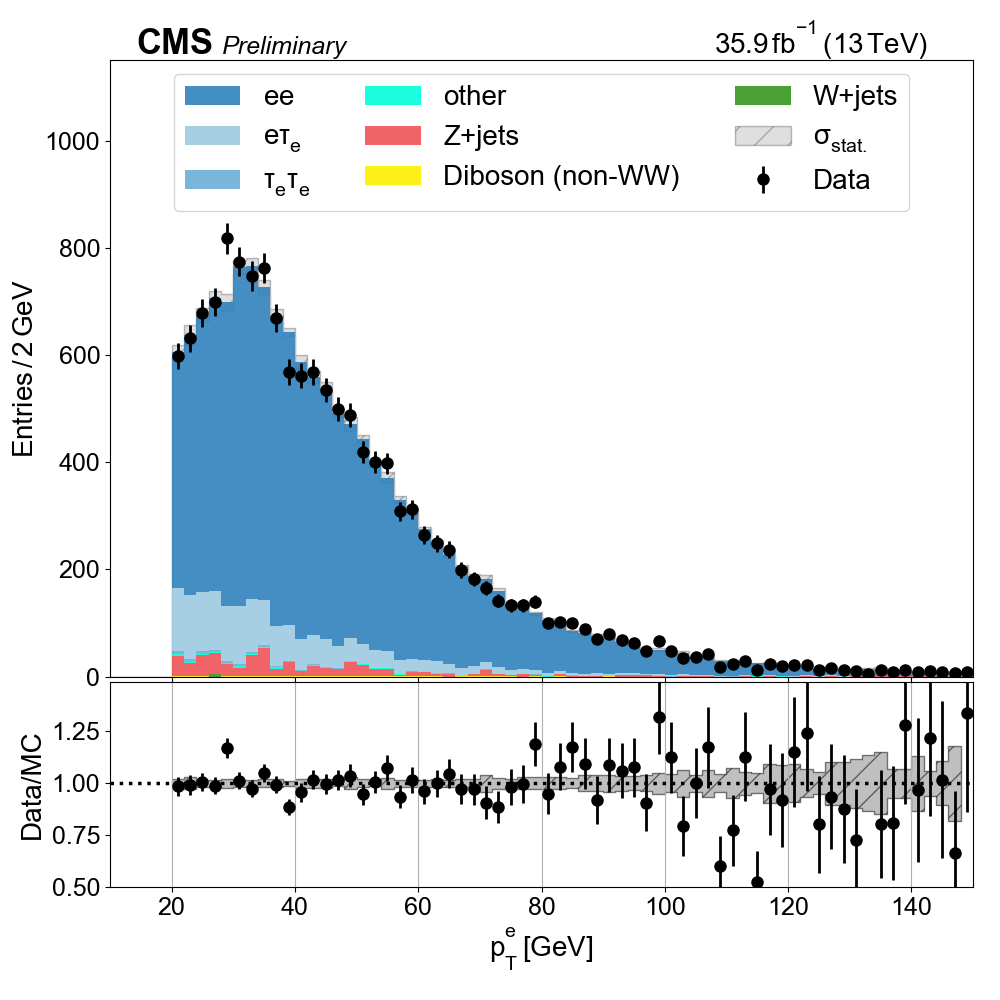
\includegraphics[width=0.4\textwidth]{chapters/Analysis/sectionPlots/figures/data_mc_overlays/ee_2016_cat_gt2_gt2_b_signal_linear_lepton_lepton2_pt}
    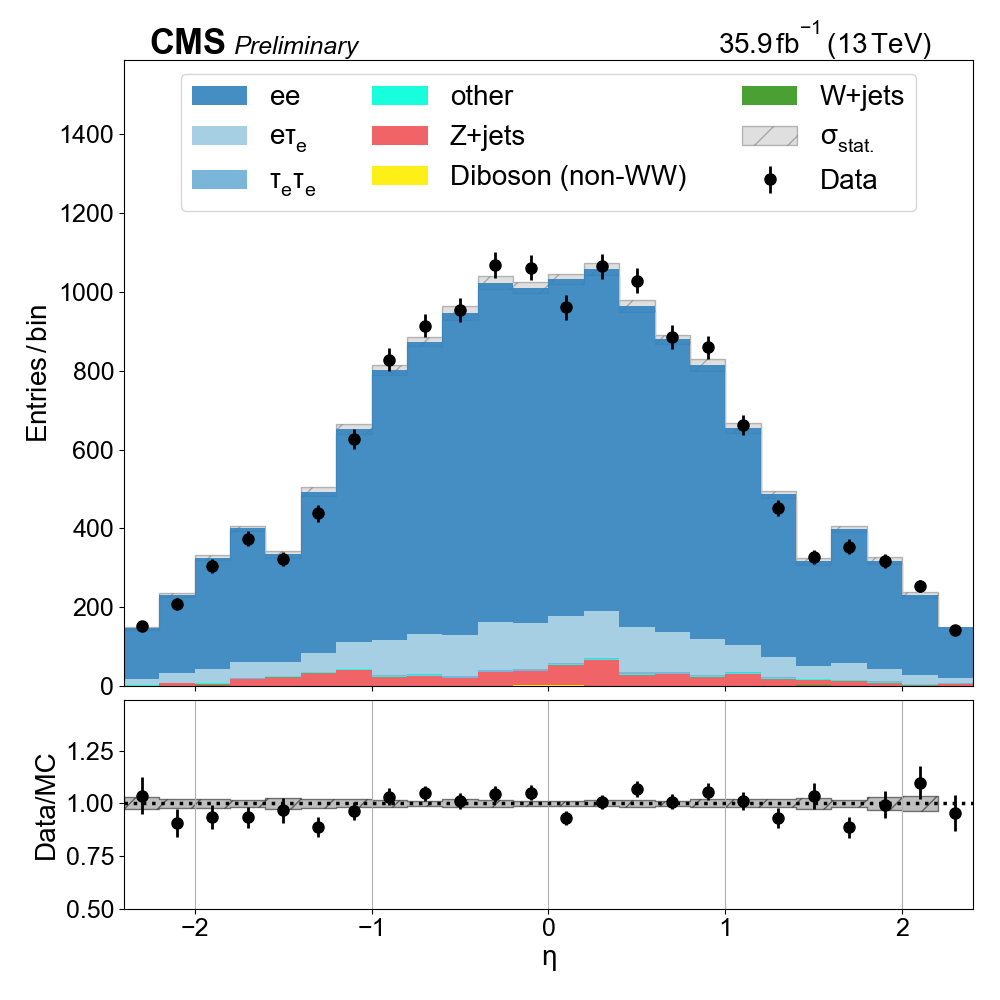
\includegraphics[width=0.4\textwidth]{chapters/Analysis/sectionPlots/figures/data_mc_overlays/ee_2016_cat_gt2_gt2_b_signal_linear_lepton_lepton2_eta}
    \caption{\pt and $\eta$ distributions for leading (top) and trailing
    (bottom) electrons in the $ee$ channel with $N_{j} \geq 2$, $N_{b}
    \geq 2$, and Z boson veto.}
    \label{fig:analysis:plots:ee_2_kinematic}
\end{figure}

\begin{figure}[htb!]
    \centering
    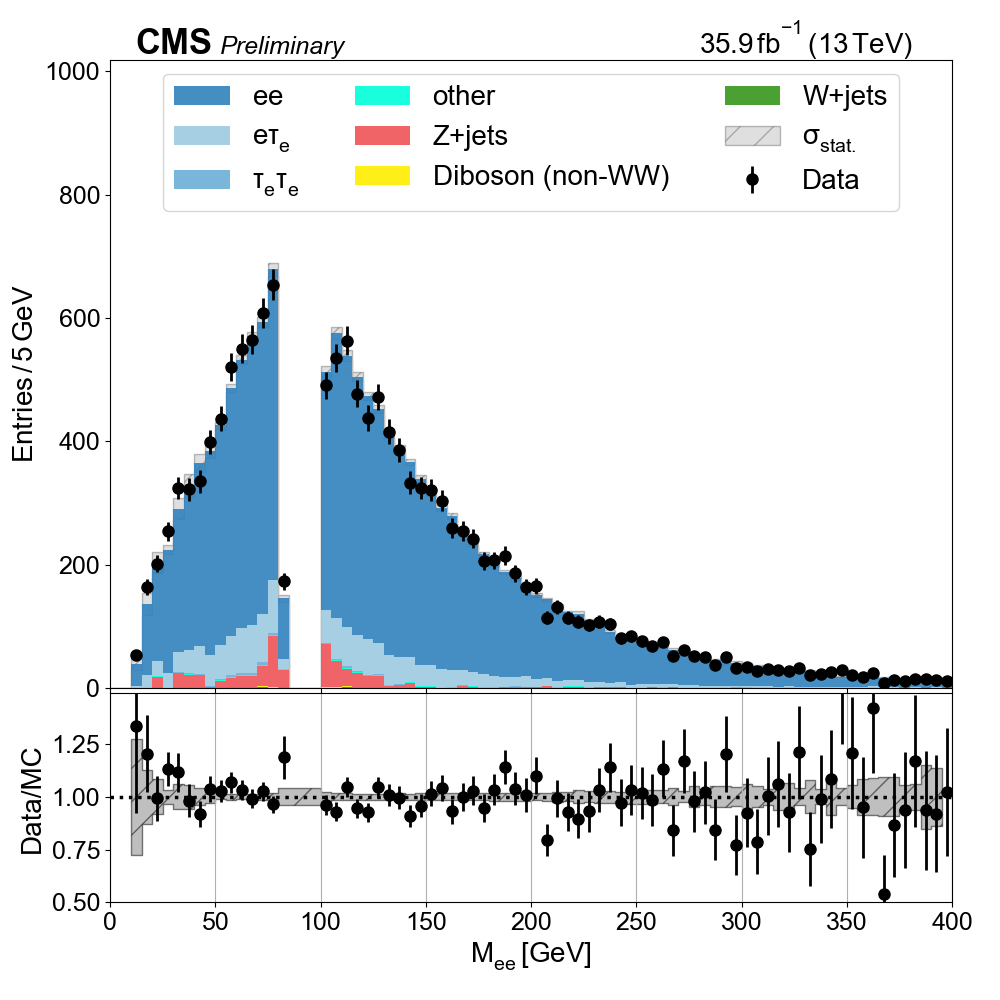
\includegraphics[width=0.3\textwidth]{chapters/Analysis/sectionPlots/figures/data_mc_overlays/ee_2016_cat_gt2_gt2_b_signal_linear_lepton_dilepton1_mass}
    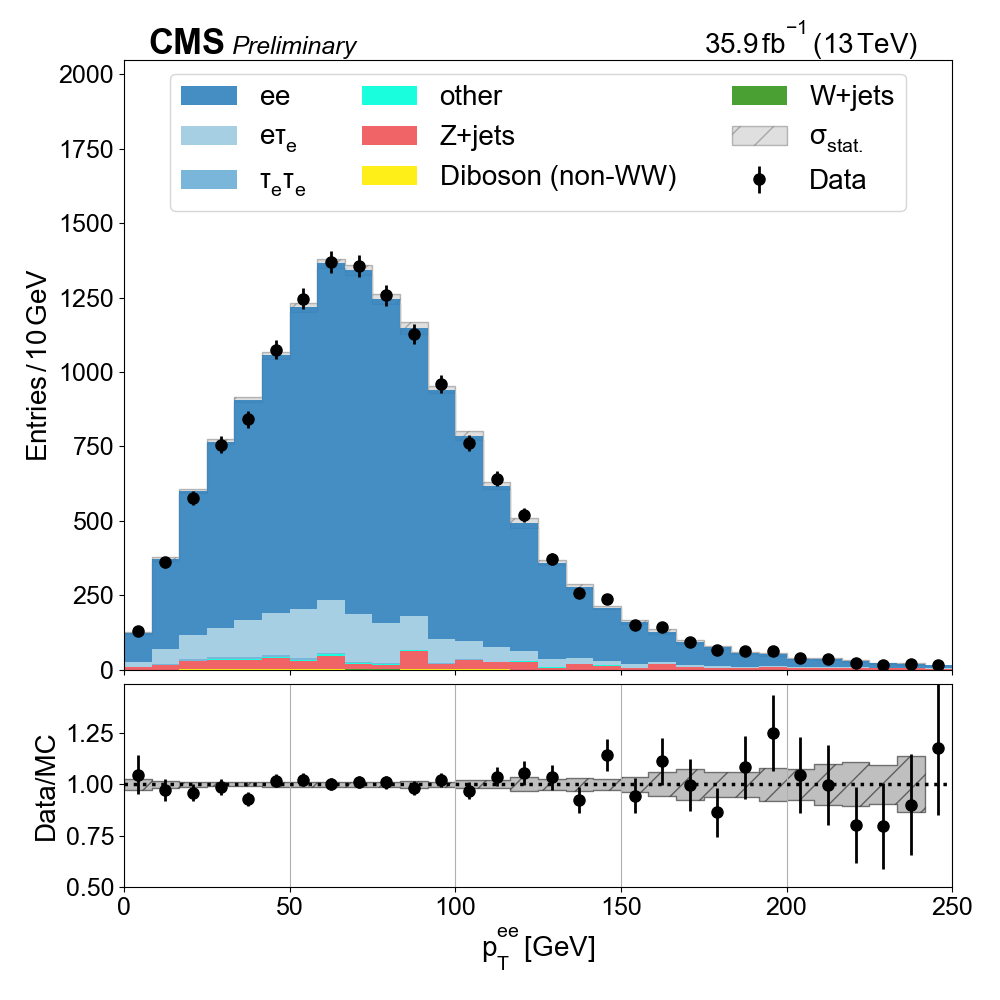
\includegraphics[width=0.3\textwidth]{chapters/Analysis/sectionPlots/figures/data_mc_overlays/ee_2016_cat_gt2_gt2_b_signal_linear_lepton_dilepton1_pt}
    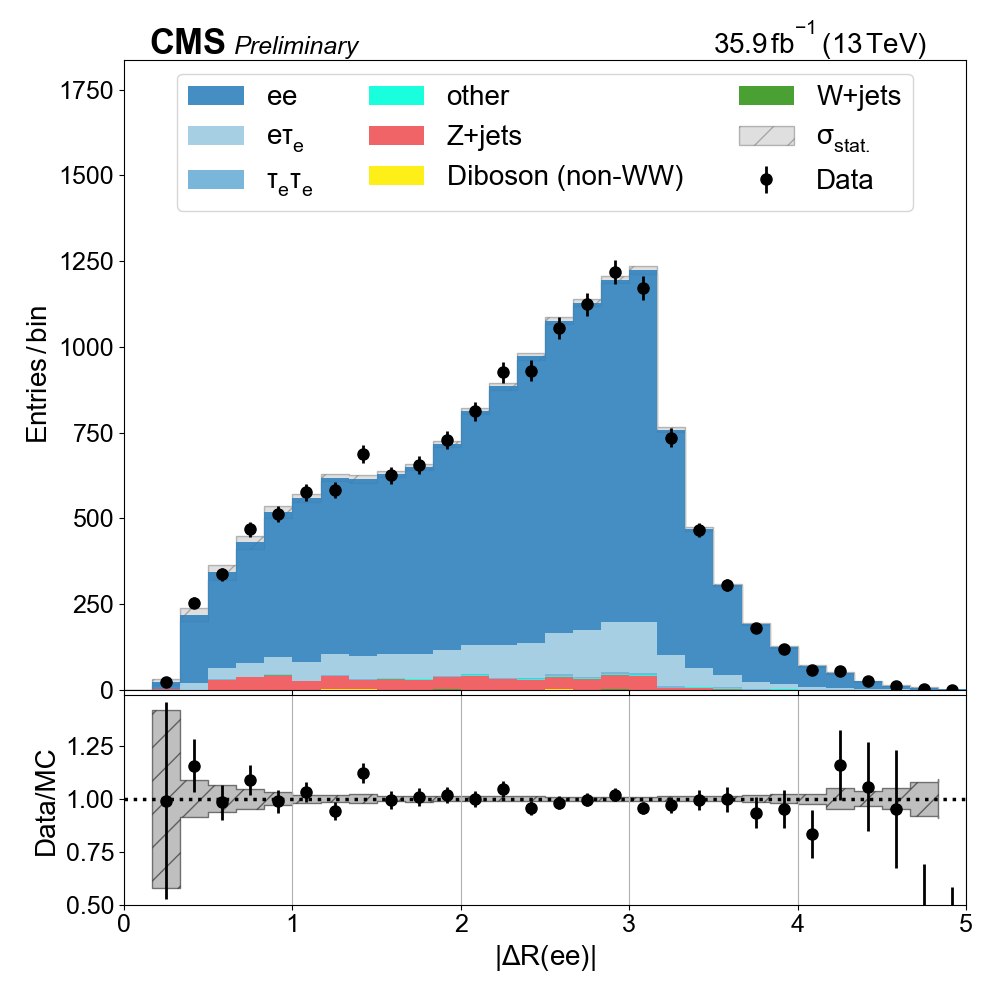
\includegraphics[width=0.3\textwidth]{chapters/Analysis/sectionPlots/figures/data_mc_overlays/ee_2016_cat_gt2_gt2_b_signal_linear_lepton_dilepton1_delta_r}
    \caption{Dielectron mass, \pt, and $\Delta R$ in the $ee$ channel
    with $N_{j} \geq 2$, $N_{b} \geq 2$, and Z boson veto.}
    \label{fig:analysis:plots:ee_2_dilepton}
\end{figure}

\begin{figure}[htb!]
    \centering
    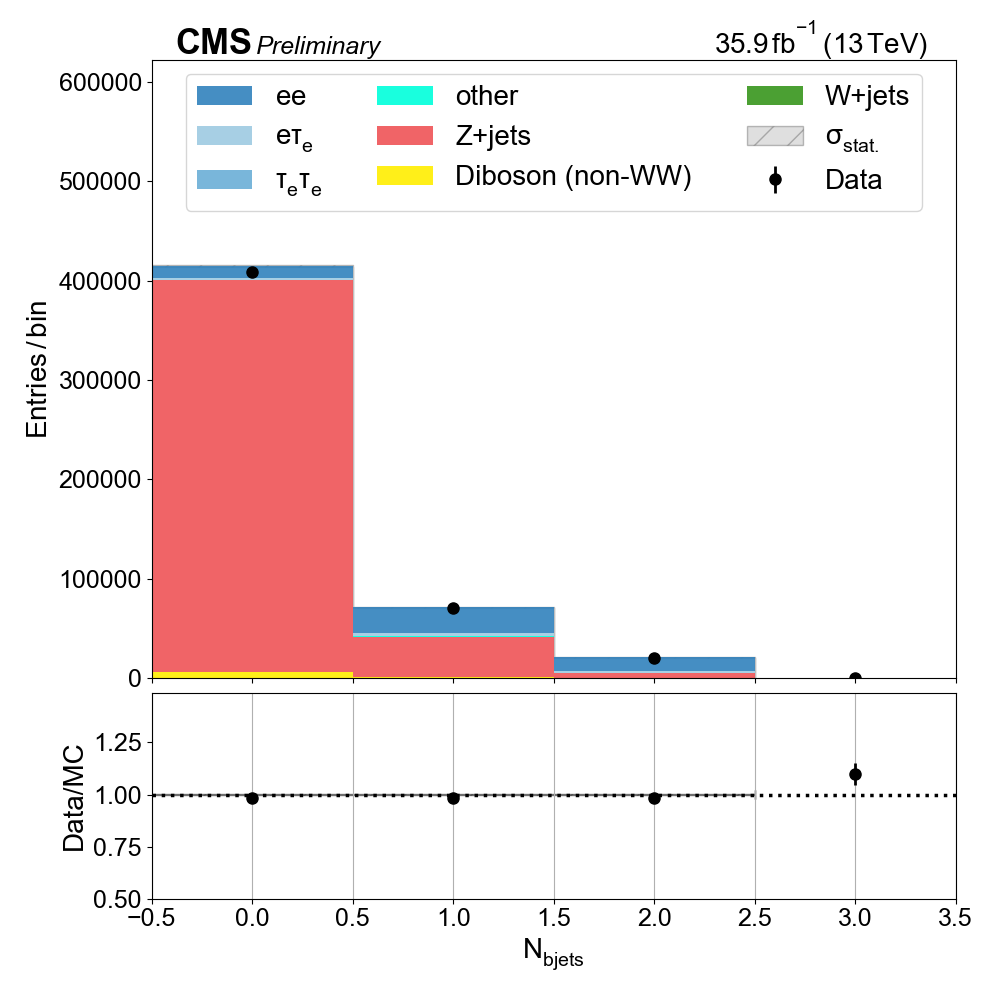
\includegraphics[width=0.4\textwidth]{chapters/Analysis/sectionPlots/figures/data_mc_overlays/ee_2016_inclusive_linear_jet_n_bjets}
    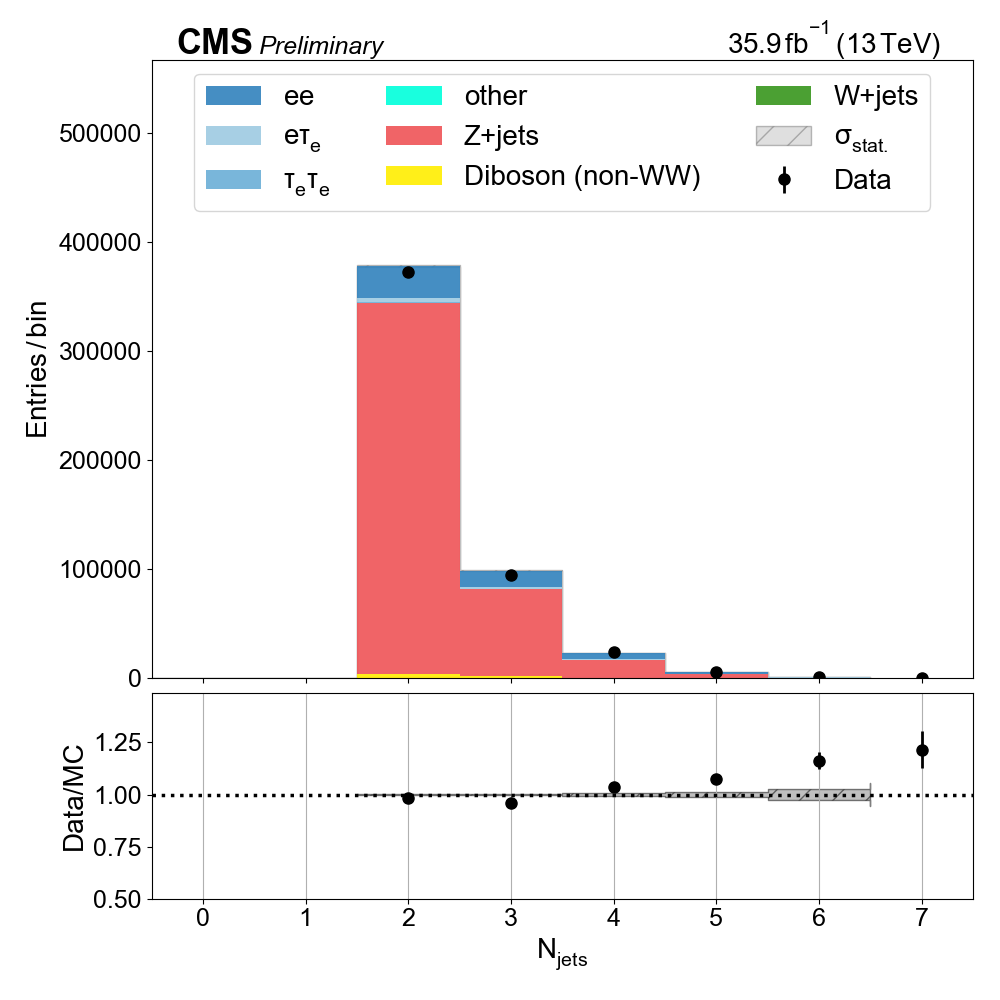
\includegraphics[width=0.4\textwidth]{chapters/Analysis/sectionPlots/figures/data_mc_overlays/ee_2016_inclusive_linear_jet_n_jets}
    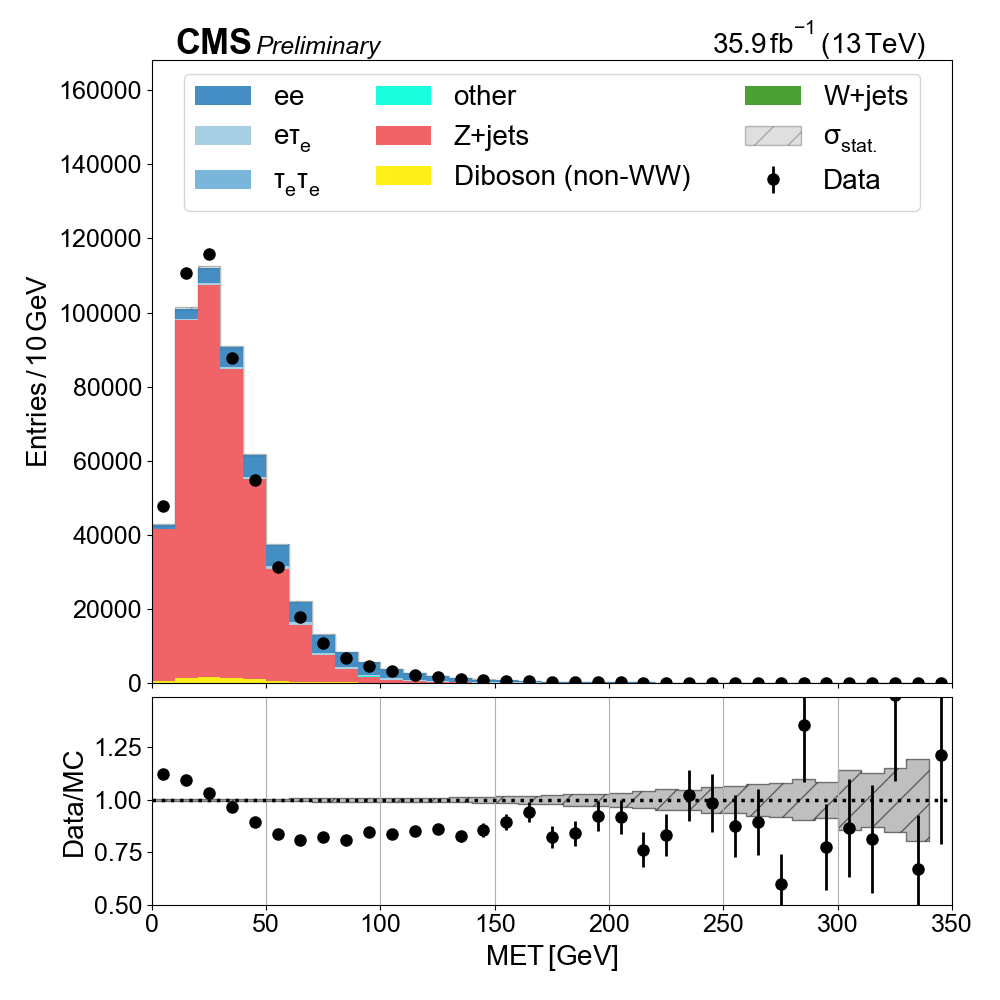
\includegraphics[width=0.3\textwidth]{chapters/Analysis/sectionPlots/figures/data_mc_overlays/ee_2016_inclusive_linear_misc_met_mag}
    \caption{Multiplicity of b tagged jets, non-tagged jets, and MET in
    $ee$ channel with $N_{j} \geq 2$.}
    \label{fig:analysis:plots:ee_jetmet}
\end{figure}

